\documentclass{article}
\usepackage[paperwidth=22.3cm,paperheight=56.3cm,margin=1.2cm]{geometry}
\usepackage{fontspec}
\setmonofont{DejaVu Sans Mono}[Scale=0.9]
\usepackage{tikz}
\usepackage{fancyvrb}
\usepackage{multicol}
\usepackage{needspace}
\usetikzlibrary{arrows.meta,decorations.pathreplacing,calc}
\definecolor{rootc}{HTML}{DCE9F7}
\definecolor{rootl}{HTML}{3B6EA5}
\definecolor{subc}{HTML}{FBE6CF}
\definecolor{subl}{HTML}{B8691B}
\definecolor{toolc}{HTML}{DDF0DD}
\definecolor{tooll}{HTML}{3F7F46}
\definecolor{gradec}{HTML}{EBDFF6}
\definecolor{gradel}{HTML}{6F4A9E}
\definecolor{ink}{HTML}{1F2328}
\definecolor{mute}{HTML}{6A737D}
\pagestyle{empty}
\setlength{\parindent}{0pt}
\newcommand{\codepage}[3]{\par\bigskip\needspace{12\baselineskip}
  {\sffamily\bfseries\large #1}\par\smallskip
  {\sffamily\small\color{mute} #2}\par\medskip
  \VerbatimInput[fontsize=\footnotesize]{#3}}
\newcommand{\topic}[1]{\par\medskip{\bfseries\normalsize #1}\par\smallskip}
\newcommand{\paper}[1]{\par\smallskip\textbf{#1}\quad}
\newcommand{\cd}[1]{{\ttfamily #1}}
\begin{document}
\color{ink}
\centering
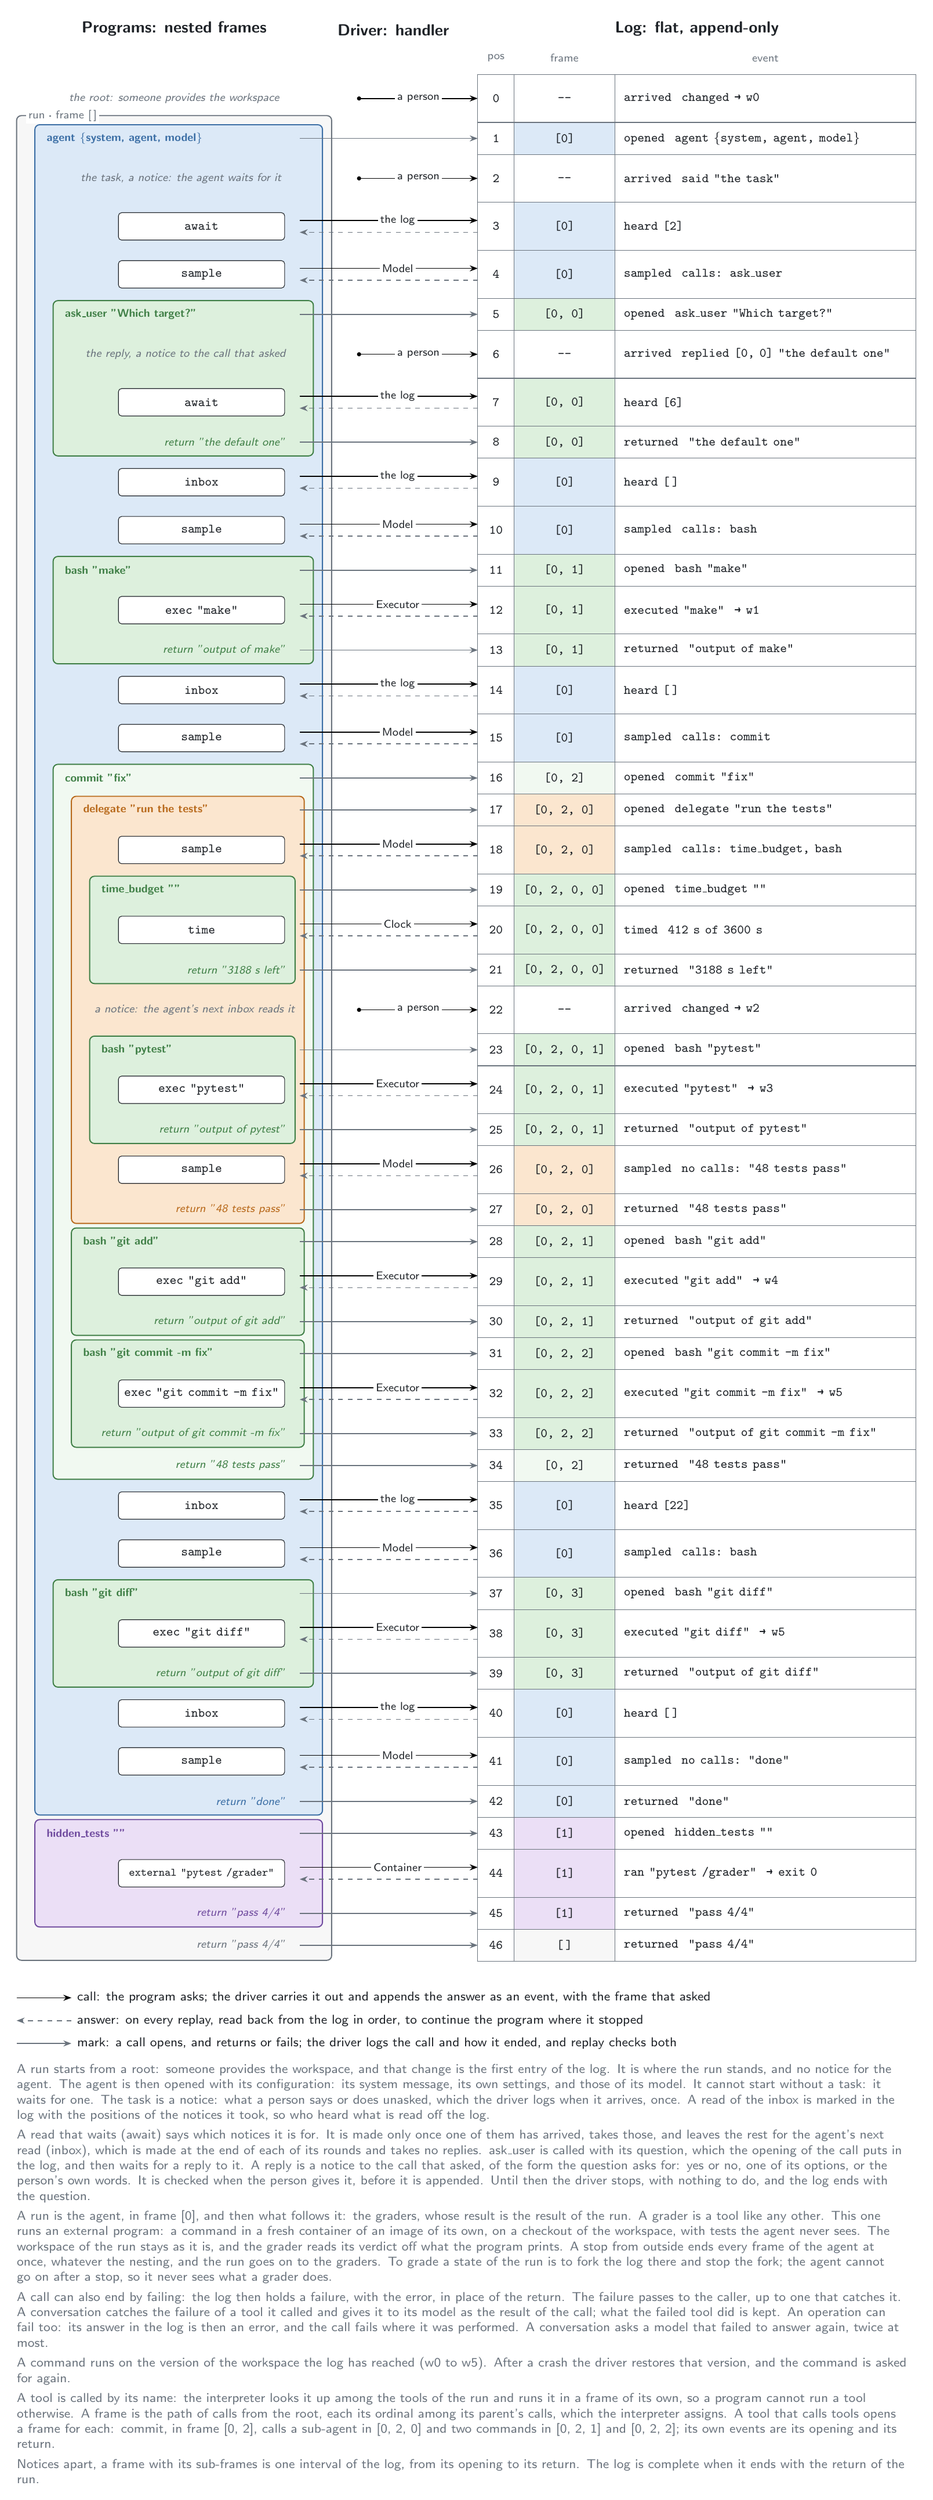
\begin{tikzpicture}[
  font=\sffamily\small, text=ink,
  op/.style={draw=ink, fill=white, rounded corners=2pt, minimum height=6mm, text width=35mm,
             align=center, font=\ttfamily\footnotesize, inner sep=2pt},
  tab/.style={fill=white, inner sep=1.5pt, font=\sffamily\scriptsize, anchor=west},
  ret/.style={fill=white, inner sep=1.5pt, font=\sffamily\scriptsize\itshape, anchor=east},
  cell/.style={draw=mute, minimum height=13mm, anchor=west, inner sep=0pt, outer sep=0pt},
  eff/.style={-{Stealth[length=5pt]}, line width=0.6pt},
  ans/.style={-{Stealth[length=5pt]}, line width=0.6pt, dashed, mute},
  hnd/.style={fill=white, inner sep=1.5pt, font=\sffamily\scriptsize},
  note/.style={font=\sffamily\scriptsize\itshape, text=mute},
]
% the height of each row of the log: the brackets of a scope are short rows
\def\ys{{0.0,-0.875,-1.75,-2.8,-3.85,-4.725,-5.6,-6.65,-7.525,-8.4,-9.45,-10.325,-11.2,-12.075,-12.95,-14.0,-14.875,-15.575,-16.45,-17.325,-18.2,-19.075,-19.95,-20.825,-21.7,-22.575,-23.45,-24.325,-25.025,-25.9,-26.775,-27.475,-28.35,-29.225,-29.925,-30.8,-31.85,-32.725,-33.6,-34.475,-35.35,-36.4,-37.275,-37.975,-38.85,-39.725,-40.425,-41.425}}
\newcommand{\Y}[1]{\ys[#1]}
% frame box: depth, the row of its opening, the row of its return, fill, line
\newcommand{\frm}[5]{%
  \draw[fill=#4, draw=#5, line width=0.7pt, rounded corners=3pt]
    ({0.4*#1}, {\Y{#2}+0.3}) rectangle ({6.9-0.2*#1}, {\Y{#3}-0.3});}
% log row: position, frame, frame fill, event, height
\newcommand{\cells}[5]{%
  \node[cell, minimum height=#5, minimum width=8mm]  at (10.1,  {\Y{#1}}) {\ttfamily\footnotesize #1};
  \node[cell, minimum height=#5, minimum width=22mm, fill=#3] at (10.9, {\Y{#1}}) {\ttfamily\footnotesize #2};
  \node[cell, minimum height=#5, minimum width=66mm, text width=62mm, align=left] at (13.1, {\Y{#1}}) {\ttfamily\footnotesize #4};}
\newcommand{\logrow}[4]{\cells{#1}{#2}{#3}{#4}{10.5mm}}
% call and answer arrows: row, handler
\newcommand{\io}[2]{%
  \draw[eff] (6.2, {\Y{#1}+0.13}) -- node[hnd, pos=0.55] {#2} (10.1, {\Y{#1}+0.13});
  \draw[ans] (10.1, {\Y{#1}-0.13}) -- (6.2, {\Y{#1}-0.13});}
% a read of the inbox: position, frame, frame fill, the positions of the notices it takes, the read
\newcommand{\readrow}[5]{\cells{#1}{#2}{#3}{heard #4}{10.5mm}
  \node[op] at (4.05, {\Y{#1}}) {#5};
  \io{#1}{the log}}
% a scope opens: position, frame, frame fill, line colour, depth, what it calls
\newcommand{\openrow}[6]{\cells{#1}{#2}{#3}{opened\ \ #6}{7mm}
  \node[anchor=west, inner sep=1.5pt, font=\sffamily\scriptsize\bfseries, text=#4] at ({0.4*#5+0.2}, {\Y{#1}}) {#6};
  \draw[eff, mute] (6.2, {\Y{#1}}) -- (10.1, {\Y{#1}});}
% a scope returns: position, frame, frame fill, line colour, value
\newcommand{\retrow}[5]{\cells{#1}{#2}{#3}{returned\ \ #5}{7mm}
  \node[ret, text=#4, fill=none] at (5.95, {\Y{#1}}) {return #5};
  \draw[eff, mute] (6.2, {\Y{#1}}) -- (10.1, {\Y{#1}});}
% a notice: row, who
\newcommand{\unasked}[2]{%
  \fill (7.5, {\Y{#1}}) circle (1.3pt);
  \draw[eff] (7.5, {\Y{#1}}) -- node[hnd, pos=0.5] {#2} (10.1, {\Y{#1}});}

% ---- frames ----
\draw[fill=black!3, draw=mute, line width=0.7pt, rounded corners=3pt]
  (0, {\Y{1}+0.5}) rectangle (6.9, {\Y{46}-0.33});
\node[tab, text=mute] at (0.2, {\Y{1}+0.5}) {run \textperiodcentered{} frame [\,]};
\frm{1}{1}{42}{rootc}{rootl}
\frm{2}{5}{8}{toolc}{tooll}
\frm{2}{11}{13}{toolc}{tooll}
\frm{2}{16}{34}{toolc!40}{tooll}
\frm{3}{17}{27}{subc}{subl}
\frm{4}{19}{21}{toolc}{tooll}
\frm{4}{23}{25}{toolc}{tooll}
\frm{3}{28}{30}{toolc}{tooll}
\frm{3}{31}{33}{toolc}{tooll}
\frm{2}{37}{39}{toolc}{tooll}
\frm{1}{43}{45}{gradec}{gradel}

% ---- operations ----
\node[note] at (3.45, {\Y{0}}) {the root: someone provides the workspace};
\node[note] at (3.6, {\Y{2}}) {the task, a notice: the agent waits for it};
\node[op] at (4.05, {\Y{4}}) {sample};
\node[note] at (3.7, {\Y{6}}) {the reply, a notice to the call that asked};
\node[op] at (4.05, {\Y{10}}) {sample};
\node[op] at (4.05, {\Y{12}}) {exec "make"};
\node[op] at (4.05, {\Y{15}}) {sample};
\node[op] at (4.05, {\Y{18}}) {sample};
\node[op] at (4.05, {\Y{20}}) {time};
\node[note] at (3.9, {\Y{22}}) {a notice: the agent's next inbox reads it};
\node[op] at (4.05, {\Y{24}}) {exec "pytest"};
\node[op] at (4.05, {\Y{26}}) {sample};
\node[op] at (4.05, {\Y{29}}) {exec "git add"};
\node[op] at (4.05, {\Y{32}}) {exec "git commit -m fix"};
\node[op] at (4.05, {\Y{36}}) {sample};
\node[op] at (4.05, {\Y{38}}) {exec "git diff"};
\node[op] at (4.05, {\Y{41}}) {sample};
\node[op, font=\ttfamily\scriptsize] at (4.05, {\Y{44}}) {external "pytest /grader"};

% ---- arrows ----
\unasked{0}{a person}
\unasked{2}{a person}
\io{4}{Model}
\unasked{6}{a person}
\io{10}{Model}
\io{12}{Executor}
\io{15}{Model}
\io{18}{Model}
\io{20}{Clock}
\unasked{22}{a person}
\io{24}{Executor}
\io{26}{Model}
\io{29}{Executor}
\io{32}{Executor}
\io{36}{Model}
\io{38}{Executor}
\io{41}{Model}
\io{44}{Container}

% ---- log ----
\logrow{0}{--}{white}{arrived\ \ changed → w0}
\openrow{1}{[0]}{rootc}{rootl}{1}{agent \{system, agent, model\}}
\logrow{2}{--}{white}{arrived\ \ said "the task"}
\readrow{3}{[0]}{rootc}{[2]}{await}
\logrow{4}{[0]}{rootc}{sampled\ \ calls: ask\_user}
\openrow{5}{[0, 0]}{toolc}{tooll}{2}{ask\_user "Which target?"}
\logrow{6}{--}{white}{arrived\ \ replied [0, 0] "the default one"}
\readrow{7}{[0, 0]}{toolc}{[6]}{await}
\retrow{8}{[0, 0]}{toolc}{tooll}{"the default one"}
\readrow{9}{[0]}{rootc}{[\,]}{inbox}
\logrow{10}{[0]}{rootc}{sampled\ \ calls: bash}
\openrow{11}{[0, 1]}{toolc}{tooll}{2}{bash "make"}
\logrow{12}{[0, 1]}{toolc}{executed "make"\ \ → w1}
\retrow{13}{[0, 1]}{toolc}{tooll}{"output of make"}
\readrow{14}{[0]}{rootc}{[\,]}{inbox}
\logrow{15}{[0]}{rootc}{sampled\ \ calls: commit}
\openrow{16}{[0, 2]}{toolc!40}{tooll}{2}{commit "fix"}
\openrow{17}{[0, 2, 0]}{subc}{subl}{3}{delegate "run the tests"}
\logrow{18}{[0, 2, 0]}{subc}{sampled\ \ calls: time\_budget, bash}
\openrow{19}{[0, 2, 0, 0]}{toolc}{tooll}{4}{time\_budget ""}
\logrow{20}{[0, 2, 0, 0]}{toolc}{timed\ \ 412 s of 3600 s}
\retrow{21}{[0, 2, 0, 0]}{toolc}{tooll}{"3188 s left"}
\logrow{22}{--}{white}{arrived\ \ changed → w2}
\openrow{23}{[0, 2, 0, 1]}{toolc}{tooll}{4}{bash "pytest"}
\logrow{24}{[0, 2, 0, 1]}{toolc}{executed "pytest"\ \ → w3}
\retrow{25}{[0, 2, 0, 1]}{toolc}{tooll}{"output of pytest"}
\logrow{26}{[0, 2, 0]}{subc}{sampled\ \ no calls: "48 tests pass"}
\retrow{27}{[0, 2, 0]}{subc}{subl}{"48 tests pass"}
\openrow{28}{[0, 2, 1]}{toolc}{tooll}{3}{bash "git add"}
\logrow{29}{[0, 2, 1]}{toolc}{executed "git add"\ \ → w4}
\retrow{30}{[0, 2, 1]}{toolc}{tooll}{"output of git add"}
\openrow{31}{[0, 2, 2]}{toolc}{tooll}{3}{bash "git commit -m fix"}
\logrow{32}{[0, 2, 2]}{toolc}{executed "git commit -m fix"\ \ → w5}
\retrow{33}{[0, 2, 2]}{toolc}{tooll}{"output of git commit -m fix"}
\retrow{34}{[0, 2]}{toolc!40}{tooll}{"48 tests pass"}
\readrow{35}{[0]}{rootc}{[22]}{inbox}
\logrow{36}{[0]}{rootc}{sampled\ \ calls: bash}
\openrow{37}{[0, 3]}{toolc}{tooll}{2}{bash "git diff"}
\logrow{38}{[0, 3]}{toolc}{executed "git diff"\ \ → w5}
\retrow{39}{[0, 3]}{toolc}{tooll}{"output of git diff"}
\readrow{40}{[0]}{rootc}{[\,]}{inbox}
\logrow{41}{[0]}{rootc}{sampled\ \ no calls: "done"}
\retrow{42}{[0]}{rootc}{rootl}{"done"}
\openrow{43}{[1]}{gradec}{gradel}{1}{hidden\_tests ""}
\logrow{44}{[1]}{gradec}{ran "pytest /grader"\ \ → exit 0}
\retrow{45}{[1]}{gradec}{gradel}{"pass 4/4"}
\retrow{46}{[\,]}{black!3}{mute}{"pass 4/4"}

% ---- headers ----
\node[font=\sffamily\bfseries, anchor=south] at (3.45, 1.25) {Programs: nested frames};
\node[font=\sffamily\bfseries, anchor=south] at (8.25, 1.25) {Driver: handler};
\node[font=\sffamily\bfseries, anchor=south] at (14.9, 1.25) {Log: flat, append-only};
\node[font=\sffamily\scriptsize, text=mute, anchor=south] at (10.5, 0.68) {pos};
\node[font=\sffamily\scriptsize, text=mute, anchor=south] at (12.0, 0.68) {frame};
\node[font=\sffamily\scriptsize, text=mute, anchor=south] at (16.4, 0.68) {event};

% ---- legend ----
\draw[eff] (0, {\Y{47}-0.15}) -- ++(1.2,0) node[right, font=\sffamily\footnotesize]
  {call: the program asks; the driver carries it out and appends the answer as an event, with the frame that asked};
\draw[ans] (1.2, {\Y{47}-0.65}) -- ++(-1.2,0);
\node[right, font=\sffamily\footnotesize] at (1.2, {\Y{47}-0.65})
  {answer: on every replay, read back from the log in order, to continue the program where it stopped};
\draw[eff, mute] (0, {\Y{47}-1.15}) -- ++(1.2,0) node[right, font=\sffamily\footnotesize, text=ink]
  {mark: a call opens, and returns or fails; the driver logs the call and how it ended, and replay checks both};
\node[anchor=north west, font=\sffamily\footnotesize, text=mute, text width=19.5cm, align=left,
      inner sep=0pt] at (0, {\Y{47}-1.6})
  {\hyphenpenalty=10000 A run starts from a root: someone provides the workspace, and that
   change is the first entry of the log. It is where the run stands, and no notice for the
   agent. The agent is then opened with its configuration: its system message, its own
   settings, and those of its model. It cannot start without a task: it waits for one. The task is a notice: what a person says or does unasked, which the
   driver logs when it arrives, once. A read
   of the inbox is marked in the log with the positions of the notices it took, so who heard what
   is read off the log.\\[3pt]
   A read that waits (await) says which notices it is for. It is made only once one of them
   has arrived, takes those, and leaves the rest for the agent's next read (inbox), which is
   made at the end of each of its rounds and takes no replies. ask\_user is called with its
   question, which the opening of the call puts in the log, and then waits for a reply to it.
   A reply is a notice to the call that asked, of the form the question asks for: yes or no,
   one of its options, or the person's own words. It is checked when the person gives it,
   before it is appended. Until then the driver stops, with nothing to do, and the log ends
   with the question.\\[3pt]
   A run is the agent, in frame [0], and then what follows it: the graders, whose result is the
   result of the run. A grader is a tool like any other. This one runs an external program: a
   command in a fresh container of an image of its own, on a checkout of the workspace, with
   tests the agent never sees. The workspace of the run stays as it is, and the grader reads
   its verdict off what the program prints. A stop from outside ends every frame of the agent
   at once, whatever the nesting, and the run goes on to the graders. To grade a state of the
   run is to fork the log there and stop the fork; the agent cannot go on after a stop, so it
   never sees what a grader does.\\[3pt]
   A call can also end by failing: the log then holds a failure, with the error, in place of
   the return. The failure passes to the caller, up to one that catches it. A conversation
   catches the failure of a tool it called and gives it to its model as the result of the
   call; what the failed tool did is kept. An operation can fail too: its answer in the log
   is then an error, and the call fails where it was performed. A conversation asks a model
   that failed to answer again, twice at most.\\[3pt]
   A command runs on the version of the workspace the log has reached (w0 to w5). After a crash
   the driver restores that version, and the command is asked for again.\\[3pt]
   A tool is called by its name: the interpreter looks it up among the tools of the run and
   runs it in a frame of its own, so a program cannot run a tool otherwise. A frame is the
   path of calls from the root, each its ordinal among its parent's calls, which the
   interpreter assigns. A tool that calls tools opens a frame for each:
   commit, in frame [0, 2], calls a sub-agent in [0, 2, 0] and two commands in [0, 2, 1] and
   [0, 2, 2]; its own events are its opening and its return.\\[3pt]
   Notices apart, a frame with its sub-frames is one interval of the log, from its opening to
   its return. The log is complete when it ends with the return of the run.};
\end{tikzpicture}

\raggedright
\newpage
\codepage{1. Programs and the log}{A signature of operations, a program as a tree over it, and
  the events of the log.}{Core.lean}
\codepage{2. Operations, tools, sub-agents and the agent}{The agent's operations, and the tools of
  a run, which programs call by name: commands, questions, sub-agents and the agent
  itself.}{Programs.lean}
\codepage{3. Replay}{The interpreter: it turns a run, the agent and what follows it, into the
  pure, total function from the log that the driver sees.}{Replay.lean}
\codepage{4. The driver}{Its loop: log what has arrived, then carry out a call and log its answer,
  or log a mark: a read of the inbox, a call that opens, a call that returns or fails.}{Driver.lean}
\codepage{5. Grading}{What follows the agent in a run: the graders. A grader runs an external
  program, in a container of its own, and reads its verdict. A state of the run is graded on a
  fork of the log that is stopped there.}{Grade.lean}
\newpage
{\sffamily\bfseries\large 6. Related work}\par\smallskip
{\sffamily\small\color{mute} Twenty-five papers read against the sketch: what corresponds, what differs, and
  what to take. Section numbers are the papers' own; the PDFs are in \cd{literature/}.}\par
\begin{multicols}{2}
\sffamily\small
\setlength{\parskip}{2pt}

\topic{Programs as trees of operations}

\paper{Hancock and Setzer (2000)} is the closest ancestor. A \emph{world} is a set $C$ of commands
with a family $R : C \to \mathrm{Set}$ of responses, which is the sketch's \cd{Signature}. An
I/O-tree is built from \cd{leaf} and \cd{do c p}, which are \cd{pure} and \cd{perform}; their bind
is the sketch's, clause for clause; and ``execution is an external operation rather than a constant
within type theory'', which is the driver. They call such a tree a strategy for one party in a
command/response interaction, the reading that \cd{next} makes literal. Their \S3 writes
loops by general recursion over well-founded trees, and names the price: definitional equality
and type checking become undecidable. In Lean the same route needs \cd{partial}, which makes a
definition opaque to proof. Their \S4 regains normalisation by making the loop a constructor
(\cd{while}) whose body must perform at least one command, so that every program terminates or
reaches its next command in finite time. The sketch follows \S4: \cd{iter} is the loop,
\cd{converse} is a loop whose state is the dialogue, and \cd{replay} rejects a round that
performs nothing.

\paper{Apfelmus (2010); Kiselyov and Ishii (2015)} define the same type again:
\cd{Program instr a} with \cd{Then} and \cd{Return}, and \cd{FFree f a} with \cd{Impure} and
\cd{Pure}. The name \cd{Program} has this precedent. Both warn that left-nested bind is quadratic;
Kiselyov and Ishii's remedy keeps the continuation as a type-aligned queue instead of a composed
function. That is not pressing here, since \cd{converse} binds to the right and every operation
is a model call or a command. Their open unions, with one interpreter per effect, are the
alternative to a closed signature such as \cd{Op}, and are worth the machinery only when others must add
operations. Their \cd{feedAll}, which answers requests from a list, is \cd{replay} for a single
operation, except that it fails at the end of the list where \cd{replay} returns the pending call.
On scopes they stop: ``the detailed investigation of the notion of scope deserves its own paper.''

\paper{Xia et al. (2020)} give the coinductive version, interaction trees: \cd{Ret}, \cd{Vis e k}
and a silent \cd{Tau}, so that a program that loops without performing is still a value. They note
that an inductive tree without \cd{Tau} restricts systems to acyclic ones, and that splitting
events into a type of operations and a family of answer types, as \cd{Op} does, is McBride's
``general monad''. They use the word \emph{driver} as the sketch does, for the outermost loop
outside the proof assistant. Three things apply. Their trace type (\S7) is the log: a list of
events with answers that ends in a result or in an event ``waiting for a response from the
environment''. It gives \cd{replay} a specification: \cd{done} when the log is a complete trace of
the program, \cd{ask} when the log followed by the pending call is one, \cd{mismatch} when the log
is a prefix of none. Their criterion for an interpreter is that it ``commutes with ret and
bind''. \cd{replay} returns its cursor, a position in the log with the unread notices and the call counter, so it is
a state monad over the cursor and the law can be stated. The sketch's \cd{iter} is their loop
combinator. They also give McBride's recursion-as-an-effect with a fuel semantics; for
\cd{replay} the finite log is the fuel. In their related work, CertiKOS gives
a sequential component as ``a deterministic function from environment interactions (as represented
by the log) to its next action'', which is the type of \cd{next}.

\paper{McBride (2015)} has the same tree as \cd{General S T X}, with \cd{S} the requests and
\cd{T s} the responses: ``request-response trees''. His subject is recursion. A recursive function
is written as one total step in which every recursive call is a request, and how to run it is
chosen afterwards: with a supply of fuel (``petrol''), coinductively, or with a domain predicate.
The sketch's \cd{round} is such a step, with the loop as a constructor in place of a call
request. Every round performs a \cd{sample}, so against a finite log the number of rounds is
bounded by the length of the log, and \cd{replay} needs no other fuel. A tool is called in
the same way: the sketch's \cd{call} is a request that names the tool and holds no body, so it
is data, and the log holds it as the opening of the call. The interpreter answers it by running
the tool the run has under that name; how deep calls nest is bounded by fuel, the length of the
log again, since a body is entered only once its opening is logged.

\paper{Pir\'og and Gibbons (2014)} study the monad of trees that may be infinite, and show that a
guarded recursive equation, one in which every step performs an operation before it recurses, has
a unique solution. That is the semantic justification for a looping \cd{converse}. Read the other
way, \cd{next} is such an equation with logs as its states: from a log it gives the outcome, or an
operation whose answers lead to longer logs. The paper assumes the infinite trees exist and does
not say how to obtain them in a proof assistant.

\topic{Handlers}

\paper{Plotkin and Power (2003)} say what makes an operation algebraic: it commutes with
evaluation contexts, $E[\mathrm{op}(N, x.M)] \equiv \mathrm{op}(N, x.E[M])$. The \cd{perform}
clause of \cd{bind} is this equation. Their generic effect, $\mathrm{gen}\,M \equiv
\mathrm{op}(M, x.x)$, is the sketch's \cd{perform op}, which is \cd{.perform op .pure}. They
also show (Example 3) that exception handling fails the equation and is ``of a different
computational character'', a deconstructor of effects. A construct that runs a body in a
frame of its own is of that kind too: \cd{bind} would extend its continuation but not its body.
The sketch keeps it out of the syntax: \cd{call} names a tool and holds no body, so it is an
operation like \cd{perform}, and what is scoped about it is in the interpreter, which runs the
named tool in a child frame. Raising is algebraic as well, and the
sketch's \cd{fail} is that; \cd{try} and \cd{catch} are the other half, written as a function of
the whole program (\cd{attempt}).

\paper{Plotkin and Pretnar (2009)} make a handler a model of the effect theory, and handling the
unique homomorphism out of the free model. The \cd{pure} and
\cd{perform} clauses of \cd{replay} have this form. Their input-redirection handler (\S6.7), which
answers \cd{in} from the head of a list passed along as a parameter and performs the real \cd{in}
once the list is empty, is the nearest construct to \cd{replay} on this side of the literature. It
has no check that the answer belongs to the operation, and it performs where \cd{replay} stops.
Their handling construct, \cd{try t with H as x in t'}, is what the interpreter does for a
\cd{call}: it handles the body of the tool with one fixed handler, which puts the body's events
in a child frame, and goes on with the continuation.
Their correctness condition, that a
handler respect the equations of the theory, is vacuous while \cd{Op} has no equations, and
becomes an obligation once one is asserted. They
warn that parallel composition ``apparently requires a binary variant of handlers'', which bears
on running tool calls concurrently.

\topic{Scopes}

\paper{Wu, Schrijvers and Hinze (2014)} show that when a handler also delimits a scope, the order
of handlers and the extent of the scope cannot be chosen independently. They give two remedies:
begin and end markers in the syntax (\S7), and higher-order syntax in which the operation carries
the computation (\S10), as in \cd{Catch (m x) (e -> m x) (x -> m a)}. \cd{call tool k} is the
second with the computation replaced by its name: the body is the tool the run has under that
name, and \cd{bind} extends only the continuation, as their \cd{emap} does. They conclude that higher-order syntax is ``strictly more expressive'' and that
markers ``run the risk of being unbalanced''. The log has both: every event carries its whole
frame path, and a call is bracketed by an \cd{opened} event, which is the call, and a
\cd{returned} event, which holds what the tool gave. \cd{replay} knows both in advance and
checks the logged ones against them, so the markers cannot be out of place, and a tool that
performs nothing still shows. A scope that means more than a frame is their \cd{Catch}, a
scope with a handler argument, and a \cd{call} is one: it catches the failure of its tool and
gives its continuation the value or the error, and the log marks which. Their example
poses the question such a design faces, whether the effects inside a failed scope are kept or
rolled back; for an append-only log they are kept. A \cd{stopped} event from outside is a failure
that nothing in the agent catches: it ends every frame of the agent, and the run goes on with
what follows. Timeouts and joining
parallel siblings are not in the paper.

\paper{Pir\'og, Schrijvers, Wu and Jaskelioff (2018)} give the formal account. In their monad of
scoped syntax a scoped operation is a pair of the computation in the scope and a continuation,
with the type between them hidden. \cd{Program} is not this monad: a \cd{call} holds the name of
its computation and not the computation, so the two are paired by the interpreter. What a run
leaves is their flat form all the same. Their Theorem 5.1 shows that the nested syntax is isomorphic to a flat one
with matched opening and closing brackets, which justifies storing a run as a flat log; the
sketch's \cd{opened} and \cd{returned} events are those brackets. An
interpreter of scoped syntax is a \emph{scoped algebra}: besides the operations it says how to
enter a scope (promote) and how to leave one (demote), at every depth. The \cd{call} clause of
\cd{replay} fits as a state-passing instance: enter with the child frame and a counter of zero,
leave by continuing the parent with its counter plus one. Their index is the depth of nesting
only; a path such as \cd{Frame}, and several kinds of scope, are future work there.

\paper{Bach Poulsen and van der Rest (2023)} generalise to operations with any number of
computation parameters (hefty trees), whose bind extends ``continuations (but not computation
parameters)'', as \cd{Program.bind} does for the rounds of a loop. Meaning comes in two stages: an \emph{elaboration}
turns each higher-order operation into ordinary operations and handlers, and handlers then
interpret the result. Laws are stated and proved for an elaboration together with a handler, not
for the syntax. For a \cd{call}, the elaboration that matches the log is a handler applied to
the tool's body that puts its events in a child frame, and its laws hold only up to renumbering,
since a tool that does nothing still consumes an ordinal and logs its brackets. Their two
elaborations of \cd{catch}, one keeping the effects of the failed block and one rolling them
back, are the choice for a failed call; the sketch keeps them. Their
\cd{spawn} elaborates to an interleaving, which strict in-order matching would not accept.

\topic{Replay}

\paper{Koppel, Scherer and Solar-Lezama (2018)} obtain a continuation by ``replaying the entire
computation from the start, guiding it using a recording''. Their past and future stacks are the
consumed and the remaining log, and the replayed computation is constant, like the program given
to \cd{next}. Their Theorem A.5 (a replayed configuration reduces back to the original by pure
steps) and Lemma A.3 (appending to the future preserves those steps) are the two theorems the
sketch should have. The difference is why replay is needed. They replay because a direct-style
language cannot hand over the continuation, and say that languages with monad syntax ``may not
benefit''. The sketch already holds the continuation, as \cd{k} in \cd{perform op k}, and replays
only because \cd{k} is not persisted. So a live driver should continue with \cd{k} and replay only
after a restart, which is their optimisation of \S6.2 and removes the quadratic cost. They require
that the replayed computation have no other side effects but do not check it; \cd{mismatch} is the
check. Of persisted logs they say only that replay logs in web frameworks ``are equivalent to
serializing a continuation'', which is the architecture in one sentence.

\paper{Burckhardt et al. (2021)} formalise Durable Functions. An orchestration is deterministic
code that is replayed; nondeterminism and I/O ``must be wrapped in an activity, to ensure it is
properly recorded and replayed''. So orchestration, history and activity are program, log, and
\cd{sample} or \cd{exec}. Their main result (Theorem 6.4) is that persisting histories is
bisimilar to persisting intermediate states, with determinism isolated in one lemma: a fault-free
reference model and a proof that the implementation simulates it, the form in which to state the
sketch's correctness. They differ from the sketch in four ways. The history records a request
when it is issued and its response when it arrives, as two entries matched by a fresh
identifier, not by position, which is what permits fan-out and fan-in. Replay happens once per
work item and is followed by live execution, not once per operation. History growth is named as
a problem, with two remedies: sub-orchestrations with histories of their own, and
\cd{continue\_as\_new}, which restarts with a value and replaces the history by one entry;
compacting the dialogue is the natural point for it in an agent. And the crash window is closed
only for internal state, by committing the new history atomically with the input it consumed:
``external calls can be duplicated if there are multiple attempts at executing a work item.''
\cd{exec} needs its own answer: the sketch runs a command on the version of the workspace the
log has reached, so that a command run again after a crash starts from the same workspace. The paper has no runtime check for nondeterminism, no
versioning of code against existing histories, and no messages delivered into a running
orchestration, so nothing corresponding to \cd{inbox}.

\paper{Thiemann (2002)} is the earliest instance found of the whole scheme. A WASH/CGI script is
re-run from the start on every request, with ``a log of the responses from the user and from I/O
operations'', and ``each input operation tries to get its result from the front of the first
queue. Only if the queue is empty it performs the actual input.'' The justification is the
sketch's: in a pure language ``all other values can be recomputed with equal outcomes''. The log
holds answers only, with no record of which operation each one answers, so the check behind
\cd{mismatch} is an addition of the sketch. The log travels in the page, so every page is a prefix
that can be continued, which is forking a run. For state outside the program he uses time-stamped
handles that detect a value that is no longer current; the versions of the workspace in the
sketch's log are such handles. His script stops at a form until the user responds. The
sketch's \cd{ask\_user} stops the same way, at a read of the inbox that waits, and the reply is a
notice to the call that asked, logged when the person gives it.

\paper{Zhang et al. (2020)} built Beldi, which re-executes a crashed function and skips the operations already
logged under an instance identifier and a step number. The authors separate cases the sketch treats
alike. A read need not be atomic with its log entry, since a lost answer costs only a second
read; that covers \cd{sample} and \cd{time}. A write must be atomic with its log entry, which
Beldi achieves with one conditional write in the database that also holds the log. A call to
another function is made exactly-once by logging the callee's identifier first and having the
callee deduplicate on it. For anything that does not cooperate, Beldi ``only guarantees that the
operation is performed at least once''. So \cd{exec} is exactly-once only if the executor records
an identifier and the output atomically with the change to the workspace. Otherwise the guarantee
to state is at-least-once. The sketch states it so: a command whose answer was not logged is run
again, on the version of the workspace the log has reached. It writes no intent before a
command, so on restart a partial effect of the command cannot be told from a change made from
outside while the driver was down, and the driver restores the logged version.

\paper{Goldstein et al. (2020)} built Ambrosia, which also replays a log of inputs. They treat input that is
pushed from outside and cannot be replayed, such as a person typing. For such an \emph{impulse}
``the arguments are recorded in the log before execution''. The sketch's \cd{arrived}
is this: the driver appends a notice when it arrives, and that is the only place the notice is
held. A read of the \cd{inbox} is logged as a mark that holds the positions of the notices it
took, so which read took a notice can be seen in the log without the program. To bound the log they checkpoint, which presupposes state that can be
serialised; in the sketch that is the dialogue at the top of a round, not a continuation. Their
upgrade recovers with the old code and converts its state at a checkpoint. It is the one
treatment of code versions found, and it avoids replaying an old log against new code.

\topic{Concurrency}

The sketch is sequential by decision: one call at a time, matched by position. These three
papers say what parallel calls would take.

\paper{Gu et al. (2018)} is the source of the CertiKOS sentence above. All participants append
events to one global log; a participant's ``strategy $\varphi_i$ is a deterministic partial
function from the current log $l$ to its next move''; and \emph{replay functions} ``reconstruct
the current shared state from the log''. The events of others are not skipped. A thread is given
its meaning relative to an environment context $E$, and the machine ``repeatedly asks $E$ for
environmental events until the control is transferred to $i$''. For parallel calls this is the
model: when one frame is replayed, events of other frames are environment events at each
\cd{perform}, not a \cd{mismatch}, and what participants may assume of each other is an invariant
over the log. Notices are already taken so: \cd{replay} passes them on its way to the next
answer and keeps them for the \cd{inbox}. The correspondence is partial. Their replay rebuilds
shared state, not a
continuation; an event is the participant's own move, with results recomputed and not stored;
and there is no nesting.

\paper{Marlow et al. (2014)} built Haxl, in which a monadic program exposes every request it is
blocked on.
A blocked result carries a sequence of requests and the rest of the computation; \cd{<*>}
explores both of its arguments and joins their requests, where \cd{>>=} cannot look past its
first. They considered and set aside the constructor \cd{Blocked (Request r) (r -> Fetch a)},
which is \cd{perform}, because with several requests the results are hard to connect to their
continuations, and used mutable references. A pure \cd{replay} has a key instead: the frame and
an ordinal within it. Their soundness argument needs requests to be reads, since ``operations in
Fetch may take place in any order''. Two \cd{exec}s in one workspace are the excluded case, and
their cache keyed by request would be wrong for \cd{exec}. Their \cd{<*>} differs from the one
that bind defines, which they concede breaks a convention; an explicit parallel constructor
avoids the question.

\paper{Chappe et al. (2023)} add nondeterministic choice nodes to interaction trees. Parallel
composition there is not a fold over the tree. It needs a function \cd{head} that computes the
actions a tree can take next, which is what a \cd{next} returning a set of calls would be; and a
scheduler is a \emph{refinement} that resolves the choices, of which a recorded log is one. Two
limits matter: nothing joins the results of parallel branches, and a question and its answer are
one step, so several outstanding requests are not modelled.

\topic{Names and reuse}

\paper{Wingate, Stuhlm\"uller and Goodman (2011)} name each random choice by its ``structural
position in the execution trace'' (the functions, line numbers and loop indices on the call
stack), so that a re-execution whose control flow has changed can look up and reuse the choices
that are unaffected. Naming choices by order of encounter they call naive: after one change the
rest of the sequence is misaligned and ``must probably be discarded''. The sketch matches by
order, and \cd{mismatch} is that misalignment. This costs nothing today, because a program is
replayed only against its own log and its control flow cannot change. Frame paths are structural
across nesting but ordinal among siblings, and they name calls, not operations. The paper's
scheme becomes necessary in two cases. If sibling calls run in parallel, their events interleave
and answers must be found by name, which needs a name per operation: the frame path and a counter
within the frame. If an old log is replayed against an edited program, their update rule is the
template: reuse an answer when the name matches and the parameters are equal, ask again
otherwise, and drop what is stale. Names stable under edits need a static component, such as the
tool-call identifier, in place of ordinals; the authors claim no optimality for their scheme.

\paper{Hammer et al. (2015)} separate two ways of matching a computation against an earlier one:
\emph{structurally}, by content, and \emph{nominally}, by a first-class name. Their example is an
insertion into a list: everything whose content transitively includes the new element fails to
match, although little changed. A \cd{sample} request that carries the whole dialogue is matched
structurally, so one early change invalidates every later request. Names given by position do no
better: they ``identify each extension by a global count'', which shifts. Their prescription is
to derive names from identities in the data, by forking the name of the input, and to keep
identity apart from validity: find the earlier result by name, reuse it if the argument is equal,
otherwise recompute and dirty what depends on it. A name used twice in one run is an error they
detect, and a poor choice of names costs reuse but never correctness.

\paper{Mokhov, Mitchell and Peyton Jones (2018)} classify build systems by what they remember. A
\emph{verifying trace} records the hashes of the dependencies used last time; a
\emph{constructive trace} ``additionally stores the resulting value''. An event of the log is
constructive in content but flat, and for them a failed verification means rebuild and carry on,
where \cd{mismatch} stops. The system nearest the sketch is one they place outside their
framework: Fabricate, ``a script that is run in-order'', later run ``from start to finish,
skipping any commands where no inputs have changed'', which they can encode only by assuming a
linear dependency between successive commands. That assumption is the sketch's strict order, and
it, not the edit itself, is why nothing after the first changed operation is reused. They also
name what cannot be cached: volatile tasks, here \cd{time}, and tasks with
untracked dependencies, as \cd{exec} would be if the versions of the workspace were not in the
log. Re-running from the start for each missing
value is their restarting scheduler; holding the continuation is the suspending one.

\paper{Cusumano-Towner et al. (2019)} built Gen, which keeps a trace as a map from hierarchical addresses to
values, where ``the address hierarchy mirrors the call hierarchy'' and the user chooses the
address at each call. \cd{update} takes a trace, new arguments and some new values, and returns a
new trace together with a \emph{discard}: the values that were overwritten or are no longer
visited. That is the operation to put in place of \cd{mismatch}, and it needs events keyed by
name. It is defined for new arguments to the same program, not for an edited program. Their
\cd{Unfold} combinator fits a loop such as \cd{converse}, but the saving is limited to the
unchanged prefix, because each round's state contains the whole dialogue.

\topic{Model calls as random choices}

\paper{Bingham et al. (2019)} say of Pyro, in this short paper, only that a program's \cd{sample}
statements are primitives ``whose behavior is overridden by inference algorithms'', and that this
is done by Poutine, a library of effect handlers. The handlers themselves, including any that
trace or replay, are not described in it.

\paper{Dohan et al. (2022)} define a cascade as ``a probabilistic program that includes
string-valued random variables, sampled from an LM''. An agent program whose control flow depends
on its samples is a cascade, and a log is one trace of it. They recast chain of thought,
verifiers, self-consistency and tool use in these terms, and use only forward sampling and
rejection. These patterns become available to the sketch once a prefix of a log can be continued
several times: sample several continuations and vote, reject and resample, or rank with a
verifier. The paper says nothing about tools with side effects when a program is run again, so
the requirement is the sketch's to state: each continuation needs its own workspace from the
point of the fork.

\topic{What the sketch takes}

\begin{enumerate}\setlength{\itemsep}{1pt}\setlength{\leftskip}{-0.6em}
\item The loop is a constructor with a state and a guard, so \cd{converse} and \cd{replay} are
  total and the log is the fuel (Hancock and Setzer \S4; Xia et al. \S4; McBride; Pir\'og and
  Gibbons).
\item \cd{replay} returns its cursor, and a log that is no trace of the program is a result of its
  own, \cd{mismatch}, not an outcome of the agent (Xia et al. \S7).
\item A command happens at least once, and runs on the version of the workspace the log has
  reached, which the driver restores on restart (Zhang et al.; Burckhardt et al.).
\item What happens unasked is logged when it arrives, once. A read of the \cd{inbox} is logged
  as a mark with the positions of the notices it took (Goldstein et al.; Gu et al.).
\item The log records the version of the workspace that each command and each change from
  outside leaves, from the root on: the workspace that someone provides, which is the first
  entry of the log (Thiemann; Mokhov et al.).
\item A tool is called by its name. The call is data, a request that the interpreter answers by
  running the tool the run has under that name in a child frame, and the log brackets it: an
  opening, which is the call, and a return with what it gave (McBride; Pir\'og et al.; Wu et al.
  \S7, \S10).
\item A tool that asks a person is called with the question and waits for a reply: a notice to
  the call that asked, of the form the question asks for, which is checked when it is appended.
  The driver stops until then, and the same loop resumes the run (Thiemann; Goldstein et al.).
\item A stop from outside ends every frame of the agent, and the run goes on with what follows
  it: the graders, whose effects the agent cannot see. A grader is a tool that runs an external
  program, an operation: a command in a fresh container of a pinned image, on a checkout of
  the workspace, which the workspace of the run does not follow. A state of a run is a prefix
  of its log, and is graded on a fork stopped there, one for each version of the workspace (Wu et al.
  \S10; Mokhov et al.).
\item A program can fail. A call catches the failure of its tool, the log marks it, and what the
  tool did is kept; \cd{try} and \cd{catch} elsewhere are a function of the program and leave
  no mark. The answer to an operation may be an error, logged like any answer, and the operation
  then fails (Plotkin and Power; Wu et al. \S10; Bach Poulsen and van der Rest).
\end{enumerate}

\topic{What it leaves}

\begin{enumerate}\setlength{\itemsep}{1pt}\setlength{\leftskip}{-0.6em}
\item The two theorems are checked on a run, at every prefix of its log, and not proved:
  \cd{replay} agrees with the trace specification, and appending the answer to the call \cd{next}
  returned continues the program where it stopped (Xia et al. \S7; Koppel et al. A.3, A.5;
  Burckhardt et al. 6.4).
\item The driver replays from the start for every call. A live driver would keep the continuation
  and replay only on restart; and since the state of a loop is data, replay could start at the
  last round, and the log be cut there (Koppel et al. \S6.2; Burckhardt et al. \S3.2, \S6;
  Goldstein et al.).
\item A failed call is not rolled back, and one sub-agent cannot be stopped from outside. A
  timeout on a call and a stop that names a frame would be further scoped operations, with laws
  stated for an elaboration (Bach Poulsen and van der Rest; Wu et al. \S10).
\item Matching is by position, so an edited program reuses nothing after its first changed
  operation. Names from identities in the data, and a discard in place of \cd{mismatch}, would
  (Hammer et al.; Cusumano-Towner et al.; Mokhov et al.; Wingate et al.).
\item Forking a run from a prefix of its log, with a workspace for each fork (Thiemann; Dohan et
  al.).
\item An intent logged before a command. Without it a command that may have run leaves no
  trace: an effect beyond the workspace can happen twice unrecorded, and a change made from
  outside while the driver was down is lost on restart (Zhang et al.).
\item An event holds the call it answers, which serves only the check behind \cd{mismatch}. For
  a \cd{sample} that is the whole dialogue, so the log grows quadratically; a hash of the call
  would serve.
\item Parallel calls, by decision (Marlow et al.; Chappe et al.; Gu et al.).
\end{enumerate}
Two questions stay open after all twenty-five. Replaying an old log against an edited program is
treated only by analogy: Gen updates a trace for new arguments, Hammer et al. for edited inputs,
and Goldstein et al. avoid the case. And none gives exactly-once execution of a command on a
target that does not cooperate; Zhang et al. and Goldstein et al. both fall back to
at-least-once.

\topic{Papers}
{\scriptsize\setlength{\parskip}{0.5pt}
P. Hancock, A. Setzer. Interactive programs in dependent type theory. CSL 2000.\par
H. Apfelmus. The operational monad tutorial. The Monad.Reader 15, 2010.\par
O. Kiselyov, H. Ishii. Freer monads, more extensible effects. Haskell 2015.\par
L. Xia et al. Interaction trees: representing recursive and impure programs in Coq. POPL 2020.\par
G. Plotkin, J. Power. Algebraic operations and generic effects. Applied Categorical Structures 11, 2003.\par
G. Plotkin, M. Pretnar. Handlers of algebraic effects. ESOP 2009.\par
N. Wu, T. Schrijvers, R. Hinze. Effect handlers in scope. Haskell 2014.\par
J. Koppel, G. Scherer, A. Solar-Lezama. Capturing the future by replaying the past. ICFP 2018.\par
S. Burckhardt et al. Durable Functions: semantics for stateful serverless. OOPSLA 2021.\par
D. Wingate, A. Stuhlm\"uller, N. Goodman. Lightweight implementations of probabilistic programming
languages via transformational compilation. AISTATS 2011.\par
C. McBride. Turing-completeness totally free. MPC 2015.\par
M. Pir\'og, J. Gibbons. The coinductive resumption monad. MFPS 2014.\par
M. Pir\'og, T. Schrijvers, N. Wu, M. Jaskelioff. Syntax and semantics for operations with scopes.
LICS 2018.\par
C. Bach Poulsen, C. van der Rest. Hefty algebras: modular elaboration of higher-order algebraic
effects. POPL 2023.\par
P. Thiemann. WASH/CGI: server-side web scripting with sessions and typed, compositional forms.
PADL 2002.\par
H. Zhang et al. Fault-tolerant and transactional stateful serverless workflows. OSDI 2020.\par
J. Goldstein et al. A.M.B.R.O.S.I.A: providing performant virtual resiliency for distributed
applications. VLDB 2020.\par
R. Gu et al. Certified concurrent abstraction layers. PLDI 2018.\par
S. Marlow, L. Brandy, J. Coens, J. Purdy. There is no fork: an abstraction for efficient,
concurrent, and concise data access. ICFP 2014.\par
N. Chappe et al. Choice trees: representing nondeterministic, recursive, and impure programs in
Coq. POPL 2023.\par
M. Hammer et al. Incremental computation with names. OOPSLA 2015.\par
A. Mokhov, N. Mitchell, S. Peyton Jones. Build systems \`a la carte. ICFP 2018.\par
M. Cusumano-Towner, F. Saad, A. Lew, V. Mansinghka. Gen: a general-purpose probabilistic
programming system with programmable inference. PLDI 2019.\par
E. Bingham et al. Pyro: deep universal probabilistic programming. JMLR 20, 2019.\par
D. Dohan et al. Language model cascades. 2022.\par}
\end{multicols}
\end{document}
